\section{はじめに}\label{ux306fux3058ux3081ux306b}

日本には様々な丼がある.
一見全国で同じような丼が作られていると考えられているが,その多くはその土地の人々の味覚,そして文化が反映された味覚マップそのものである.
しかし,昨今はCookpadのようなどの地域の人でも見ることのできるレシピサイトを参照して作られるため,全国において味の均質化が進んでいる.
それは焼肉やサラダといった,誰がどこで調理してもそれなりの美味しさを実現することができるが,最適な味ではない.
そこで必要となるのは地域と,地域に根づく特徴ある調味料の明記である.
本論文では,甘めの醤油文化が根付いた九州において美味しく調理することのできる丼を提案する.

\section{食材の選定}\label{ux98dfux6750ux306eux9078ux5b9a}

丼とは野菜,肉類,とろとろの卵が織りなす味覚相乗効果を最大限に高めるための調理法である.
人間の味覚には大きく5つ,甘味,酸味,塩味,苦味,旨味が挙げられるが,最も九州地方において特徴のある味は甘味と旨味である.
この特徴は九州の醤油にもっとも顕著に現れており,成分表示が本州の醤油とは大きく異なることからも,その特徴が確認される.
これは,寒い地方と比べて暖かい地方ではマンゴーやみかんに代表される,甘めの果実が多く実ることに関係があるかもしれないが,関係性が確かめられていない.

甘めの醤油にあう肉類としては,すき焼きに代表される牛肉が最も最初に思い浮かぶが,牛肉は高価であるため,誰でも作ることのできるレシピの材料としては不適切である.
そこで本論文では豚肉を提案する.
豚肉の頭数は鹿児島や宮崎が日本における1位と2位を占め,その潤沢な頭数から九州では値段も安い.
また,豚肉の主張しすぎない甘さ,そして旨味は丼との相性に優れる.
部位としてはバラ肉では豚肉の主張がやや突出する傾向にあるため,ロースもしくは中落ち(小間切れ)をおすすめする.

使用する調味料と野菜については,沖縄のラフテーを参考にする.
ラフテーの特徴は黒糖と泡盛の持つ深いコクと旨味である.
野菜は甘みと旨味をもたらすメイラード反応の代表例として挙げられる玉ねぎを使う\cite{maillard}.
以上の選定の結果,材料の内訳は表\ref{ta:components}に示す.
星記号の材料については,次章の調理にて詳細を述べる.

\begin{table}[ht]
\caption{材料の内訳(1人前)\label{ta:components}}
\centering
\begin{tabular}[]{@{}lc@{}}





\toprule
品目 & 分量\\
\midrule

豚薄切り肉 & 50g\\
玉ねぎ & 半玉\\
ご飯 & 0.7合\\
マヨネーズ & 大さじ1\\
☆たまご & 2個\\
☆水 & 80cc\\
☆白出汁(めんつゆでも可) & 大さじ1\\
★料理酒(泡盛が良い) & 大さじ1\\
★うまくち醤油 & 大さじ1\\
★みりん & 大さじ1\\
★黒糖(三温糖でも可) & 大さじ1\\
\bottomrule
\end{tabular}

\end{table}

\section{調理}\label{ux8abfux7406}

本章では提案する丼の調理環境および調理方法を述べる.

\subsection{調理環境}\label{ux8abfux7406ux74b0ux5883}

丼を調理するにあたって必要な調理機材は表\ref{ta:maker}に示す.
IHヒーターはガスコンロで代用可能だが,安全性の観点からIHヒーターを推奨する.
なお,IHヒーターや炊飯器のコンセントの上のホコリは出火元となるため,十分に注意して取り扱うこと.

\begin{table}[ht]
\caption{使用する調理機材\label{ta:maker}}
\centering
\begin{tabular}[]{@{}lc@{}}





\toprule
器具名 & 個数\\
\midrule

3合炊き炊飯器 & 1台\\
IHヒーター(ガスコンロ) & 1台\\
まな板 & 1枚\\
三徳包丁 & 1本\\
26cmフライパン & 1枚\\
ボール & 1つ\\
計量スプーン & 1つ\\
計量カップ & 1つ\\
キッチンペーパー & 2枚\\
\bottomrule
\end{tabular}

\end{table}

\subsection{下処理}\label{ux4e0bux51e6ux7406}

特に必須と呼べるほどの下処理はないが,豚バラ肉のくさみが気になる場合はキッチンペーパーにてドリップを拭く.
また,筋がみられる場合は三徳包丁を用いて切っておくと良い.

\subsection{食材のカット}\label{ux98dfux6750ux306eux30abux30c3ux30c8}

今回はカットする材料は玉ねぎのみであり,方法は図\ref{fig:onion}に示す.
中心を線対称に番号の手順でカットする.


\begin{figure}[ht]
\centering
\includegraphics[page=3, height=3.00000cm]{./fig/fig_bb.pdf}
\caption{玉ねぎの切り方.\label{fig:onion}}
\end{figure}

\subsection{調理手順}\label{ux8abfux7406ux624bux9806}

大まかな調理のタイムスケジュールを図\ref{fig:time}に示す.
ポイントは炊飯中の待機時間にはちょうどアニメを鑑賞できる点にある.
ジャパリパークに入園して頭をからっぽにするか,ミスター味っ子で料理魂を高めると美味しい丼が得られる関係がある.

最も重要な具の炒めと卵とじの詳細については図\ref{fig:flypan}に示す.
丼の真骨頂は旨味を引き出すメイラード反応と甘みを引き出すカラメル反応\footnote{Miller, Dennis (1998). Food Chemistry: A Laboratory Manual. Wiley-Interscience.}の究極のハーモニーにある.
美味しさを表す味皇(あじおう)計数\(\mathrm{UMAI}\)を計算すると,丼はメイラード関数とカラメル関数によって,個人経営の店1店舗を吹き飛ばす味\(\mathrm{UMAI_{zoooooooooooooooooo}}\)であることが,次式で示されている.
\begin{align}
 \mathrm{UMAI} &= \mathrm{Maillard}(\mathrm{Onion}) + \mathrm{Caramel}(\mathrm{Suger_{brown}})\\
&= \mathrm{UMAI_{zoooooooooooooooooo}}.
\end{align}

炒めの順番として,一般的には豚肉を先に炒めるが,本論文では玉ねぎを先に炒める.
これは,豚肉を先に炒めると豚肉のメイラード反応は進むが,玉ねぎのメイラード反応が完了する頃には,豚肉の水分が飛んでしまうからである.
隠し味としては,玉ねぎを炒めた後にマヨネーズを加えることで,一段コクの有る味に仕上げることができるため,おすすめする.


\begin{figure}[ht]
\centering
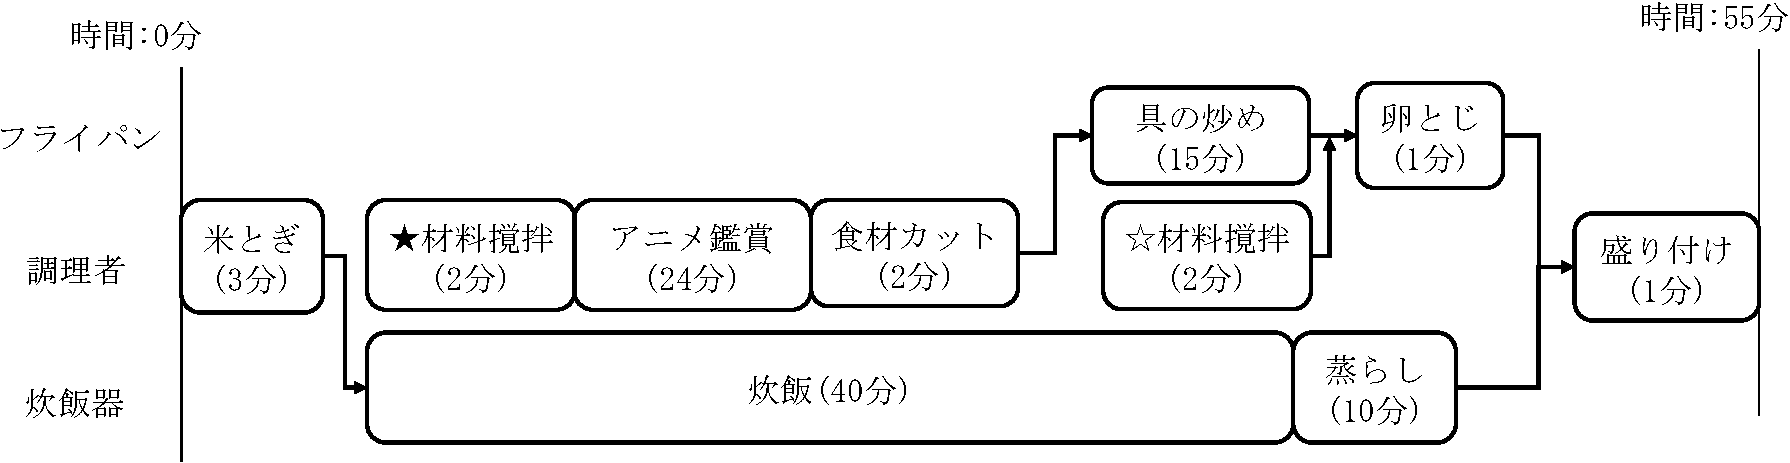
\includegraphics[page=1, width=16.00000cm]{./fig/fig_bb.pdf}
\caption{調理のタイムスケジュール.\label{fig:time}}
\end{figure}


\begin{figure}[ht]
\centering
\includegraphics[page=2, width=12.00000cm]{./fig/fig_bb.pdf}
\caption{具の炒めと卵とじの詳細.\label{fig:flypan}}
\end{figure}

\clearpage

\section{調理結果}\label{ux8abfux7406ux7d50ux679c}

本章では調理された丼を示し,考察及び今後の課題を述べる.

\subsection{調理された丼}\label{ux8abfux7406ux3055ux308cux305fux4e3c}

調理された丼は図\ref{fig:don}(a)に示す.
図\ref{fig:don}(a)ため,メイラード反応とカラメル反応の特徴である茶色の食材が確認される.
これは丼に必要な旨味と甘みを引き出す反応が十分に行われていることを意味するが,緑の色彩が失われている.
そこで画像処理(手動)によりカイワレ菜を追加したものを図\ref{fig:don}(b)に示す.
緑の色彩があったほうが丼の見た目が大幅に改善されている.
これは丼で支配的な茶色と補色関係にある色彩が緑色であるからと推測される.


\begin{figure}[ht]
\centering
\begin{tabular}[]{@{}cc@{}}

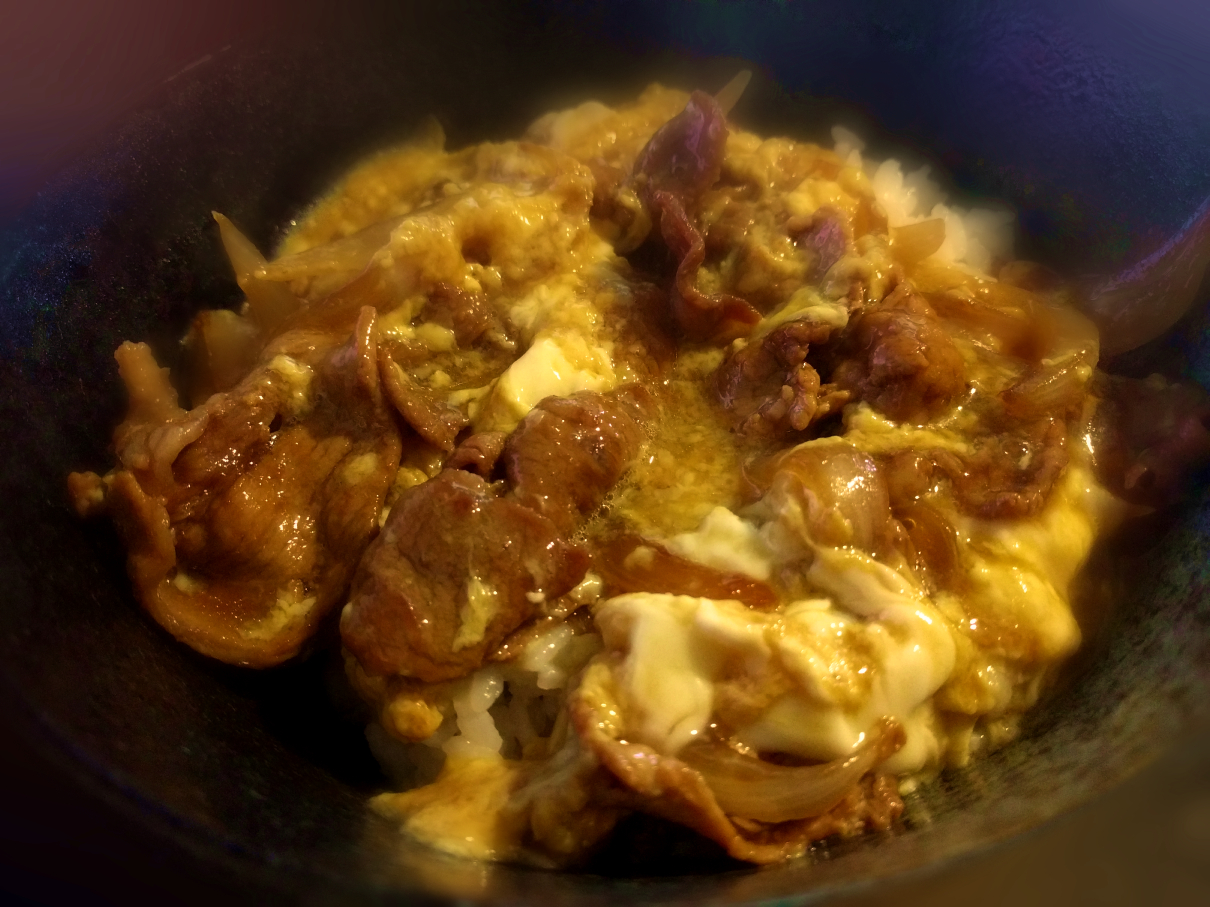
\includegraphics[width=8.00000cm]{./fig/don.jpg} &
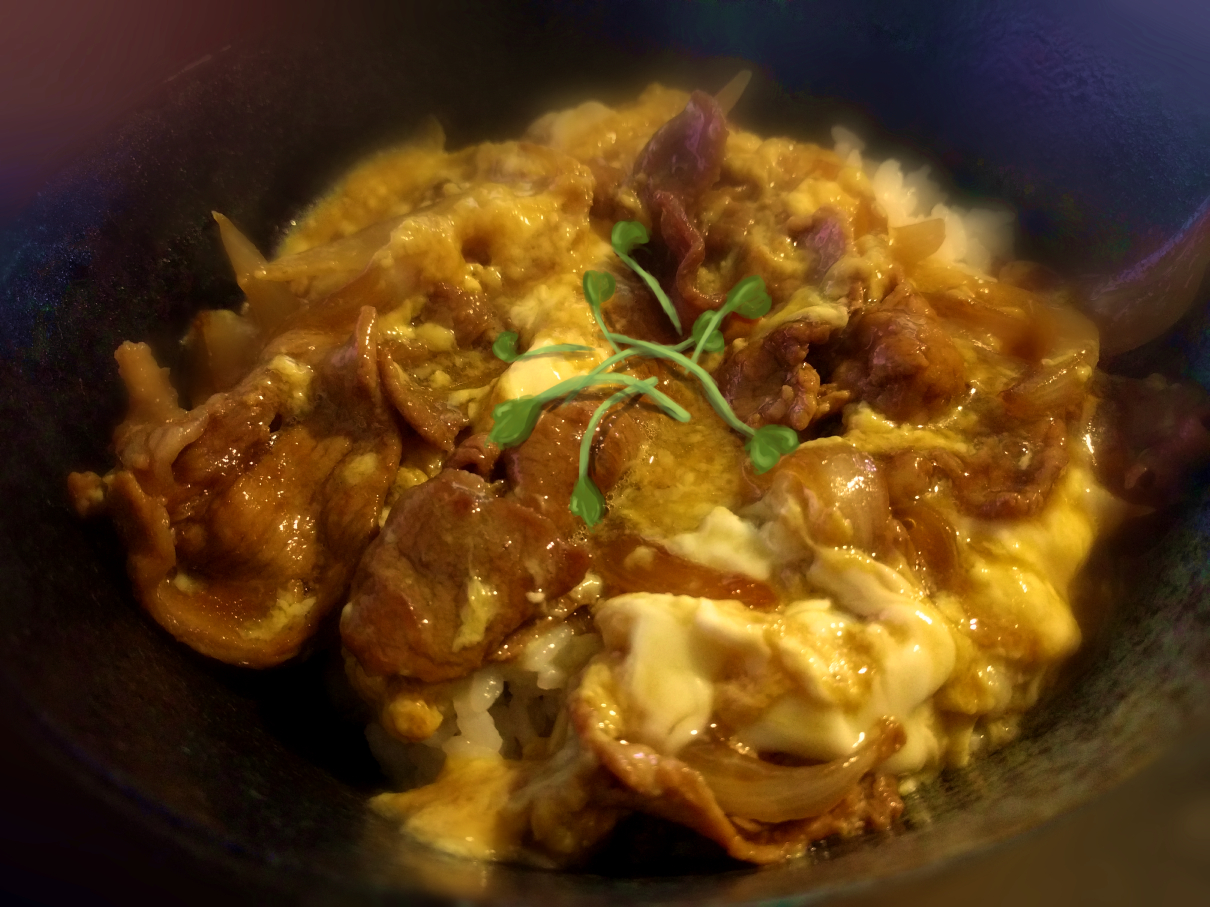
\includegraphics[width=8.00000cm]{./fig/don_green.jpg}\\
(a) & (b)\\

\end{tabular}
\caption{調理された丼の写真.(a)完成した丼,(b)色彩を追加した丼.\label{fig:don}}
\end{figure}

\subsection{丼の考察}\label{ux4e3cux306eux8003ux5bdf}

本論文で提案した丼は九州地方独特の醤油をベースに好まれる味を追求した.
これは京都のスッキリした出汁とキレのある醤油で仕上げる丼とは対象的に,甘辛さを主張する濃厚な旨味で包まれた丼だ.
著者の所感として味は申し分ないが,甘すぎるのが苦手な人は砂糖を大さじ0.5程度にするのが良い.
また,色彩が気になる人はやはりカイワレ菜や長ネギを追加するべきである.

\section{まとめ}\label{ux307eux3068ux3081}

みんなもご当地素材を使った丼を作ろう.

\begin{thebibliography}{9}
\bibitem{maillard} Maillard, L. C. (1912). "Formation of Melanoidins in a Methodical Way.", Compt. Rend. 154: 66
\end{thebibliography}

